\documentclass{standalone}
\usepackage{tikz}
\usetikzlibrary{patterns, positioning}
\usepackage[sfdefault]{ClearSans} %% option 'sfdefault' activates Clear Sans as the default text font
\usepackage[T1]{fontenc}

\begin{document}
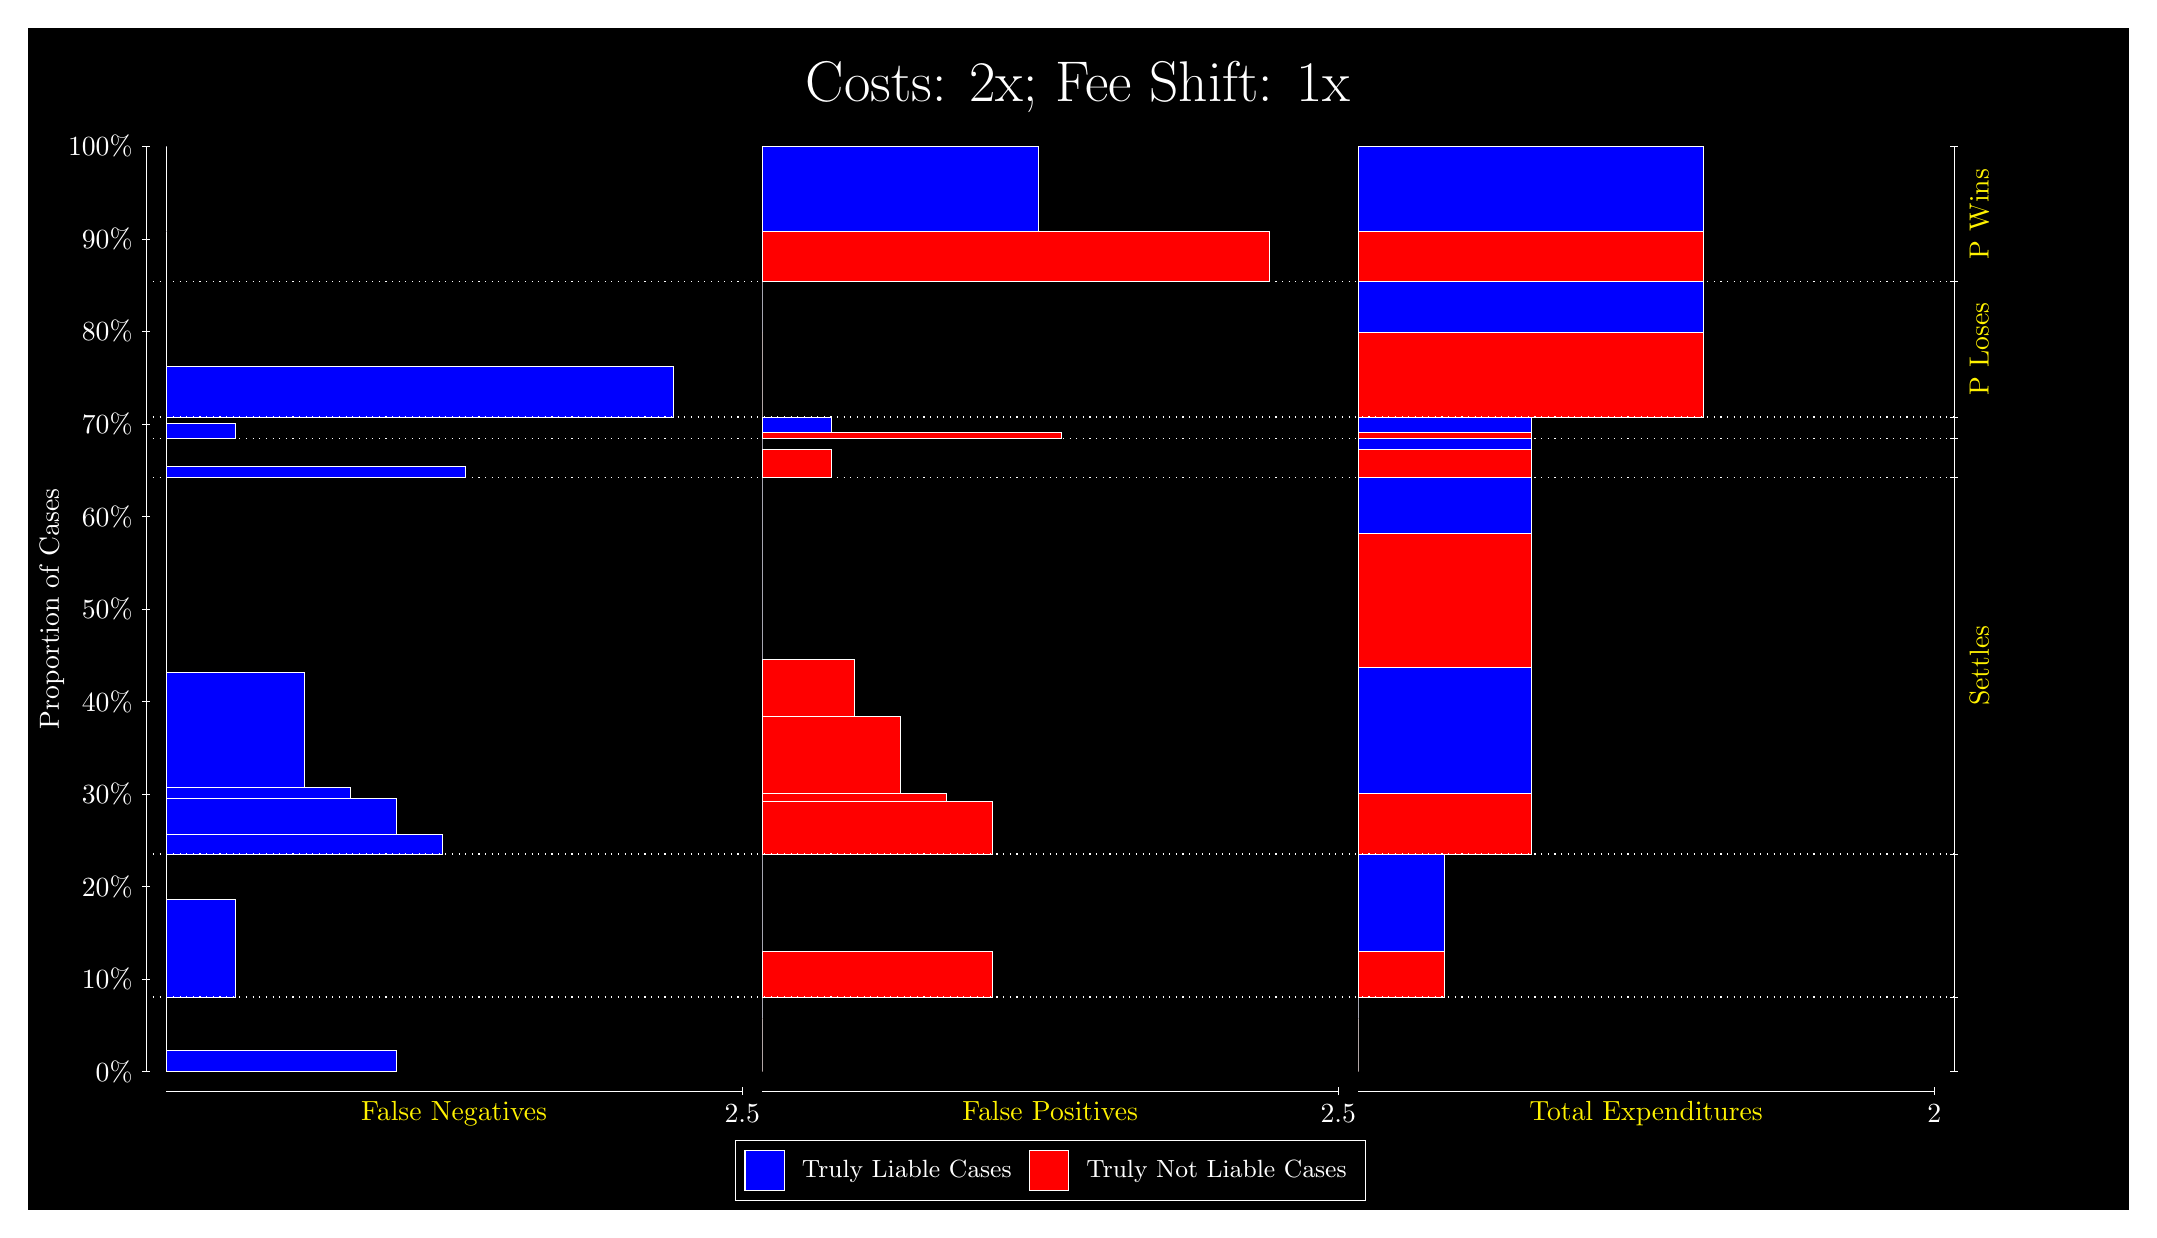
\begin{tikzpicture}
\draw[fill=black] (0,0) rectangle (26.667,15);
\draw[text=white] (0,13.5) rectangle (26.667,15) node[midway] {\huge Costs: 2x; Fee Shift: 1x};
\draw[white, very thin] (1.5,1.75) -- (1.5,13.5);
\node[rotate=90, text=white, anchor=center] at (0.3, 7.625) {Proportion of Cases};
\draw[white, very thin] (1.45,1.75) -- (1.55,1.75);
\node[text=white, anchor=east] at (1.45, 1.75) {0\%};
\draw[white, very thin] (1.45,2.925) -- (1.55,2.925);
\node[text=white, anchor=east] at (1.45, 2.925) {10\%};
\draw[white, very thin] (1.45,4.1) -- (1.55,4.1);
\node[text=white, anchor=east] at (1.45, 4.1) {20\%};
\draw[white, very thin] (1.45,5.275) -- (1.55,5.275);
\node[text=white, anchor=east] at (1.45, 5.275) {30\%};
\draw[white, very thin] (1.45,6.45) -- (1.55,6.45);
\node[text=white, anchor=east] at (1.45, 6.45) {40\%};
\draw[white, very thin] (1.45,7.625) -- (1.55,7.625);
\node[text=white, anchor=east] at (1.45, 7.625) {50\%};
\draw[white, very thin] (1.45,8.8) -- (1.55,8.8);
\node[text=white, anchor=east] at (1.45, 8.8) {60\%};
\draw[white, very thin] (1.45,9.975) -- (1.55,9.975);
\node[text=white, anchor=east] at (1.45, 9.975) {70\%};
\draw[white, very thin] (1.45,11.15) -- (1.55,11.15);
\node[text=white, anchor=east] at (1.45, 11.15) {80\%};
\draw[white, very thin] (1.45,12.325) -- (1.55,12.325);
\node[text=white, anchor=east] at (1.45, 12.325) {90\%};
\draw[white, very thin] (1.45,13.5) -- (1.55,13.5);
\node[text=white, anchor=east] at (1.45, 13.5) {100\%};

\draw[white, very thin] (24.457,1.75) -- (24.457,13.5);
\draw[white, very thin] (24.407,1.75) -- (24.507,1.75);
\node[anchor=west] at (24.407, 1.75) {};
\draw[white, very thin] (24.407,2.6964) -- (24.507,2.6964);
\node[anchor=west] at (24.407, 2.6964) {};
\draw[white, very thin] (24.407,4.5131) -- (24.507,4.5131);
\node[anchor=west] at (24.407, 4.5131) {};
\draw[white, very thin] (24.407,9.2944) -- (24.507,9.2944);
\node[anchor=west] at (24.407, 9.2944) {};
\draw[white, very thin] (24.407,9.7939) -- (24.507,9.7939);
\node[anchor=west] at (24.407, 9.7939) {};
\draw[white, very thin] (24.407,10.063) -- (24.507,10.063);
\node[anchor=west] at (24.407, 10.063) {};
\draw[white, very thin] (24.407,11.78) -- (24.507,11.78);
\node[anchor=west] at (24.407, 11.78) {};
\draw[white, very thin] (24.407,13.5) -- (24.507,13.5);
\node[anchor=west] at (24.407, 13.5) {};

\draw[white, very thin, fill=blue] (1.75,1.75) rectangle (4.6775,2.0227);
\draw[white, very thin, fill=red] (1.75,2.0227) rectangle (1.75,2.6964);
\draw[white, very thin, fill=blue] (1.75,2.6964) rectangle (2.6283,3.9339);
\draw[white, very thin, fill=red] (1.75,3.9339) rectangle (1.75,4.5131);
\draw[white, very thin, fill=blue] (1.75,4.5131) rectangle (5.2631,4.7658);
\draw[white, very thin, fill=blue] (1.75,4.7658) rectangle (4.6775,5.2236);
\draw[white, very thin, fill=blue] (1.75,5.2236) rectangle (4.092,5.3608);
\draw[white, very thin, fill=blue] (1.75,5.3608) rectangle (3.5065,6.823);
\draw[white, very thin, fill=red] (1.75,6.823) rectangle (1.75,9.2944);
\draw[white, very thin, fill=blue] (1.75,9.2944) rectangle (5.5558,9.4337);
\draw[white, very thin, fill=red] (1.75,9.4337) rectangle (1.75,9.7939);
\draw[white, very thin, fill=blue] (1.75,9.7939) rectangle (2.6283,9.9879);
\draw[white, very thin, fill=red] (1.75,9.9879) rectangle (1.75,10.063);
\draw[white, very thin, fill=blue] (1.75,10.063) rectangle (8.1906,10.702);
\draw[white, very thin, fill=red] (1.75,10.702) rectangle (1.75,11.78);
\draw[white, very thin, fill=red] (1.75,11.78) rectangle (1.75,12.417);
\draw[white, very thin, fill=blue] (1.75,12.417) rectangle (1.75,13.5);
\draw[white, very thin, fill=red] (9.3189,1.75) rectangle (9.3189,2.4237);
\draw[white, very thin, fill=blue] (9.3189,2.4237) rectangle (9.3189,2.6964);
\draw[white, very thin, fill=red] (9.3189,2.6964) rectangle (12.246,3.2756);
\draw[white, very thin, fill=blue] (9.3189,3.2756) rectangle (9.3189,4.5131);
\draw[white, very thin, fill=red] (9.3189,4.5131) rectangle (12.246,5.1794);
\draw[white, very thin, fill=red] (9.3189,5.1794) rectangle (11.661,5.2837);
\draw[white, very thin, fill=red] (9.3189,5.2837) rectangle (11.075,6.268);
\draw[white, very thin, fill=red] (9.3189,6.268) rectangle (10.49,6.9845);
\draw[white, very thin, fill=blue] (9.3189,6.9845) rectangle (9.3189,9.2944);
\draw[white, very thin, fill=red] (9.3189,9.2944) rectangle (10.197,9.6546);
\draw[white, very thin, fill=blue] (9.3189,9.6546) rectangle (9.3189,9.7939);
\draw[white, very thin, fill=red] (9.3189,9.7939) rectangle (13.125,9.8693);
\draw[white, very thin, fill=blue] (9.3189,9.8693) rectangle (10.197,10.063);
\draw[white, very thin, fill=red] (9.3189,10.063) rectangle (9.3189,11.141);
\draw[white, very thin, fill=blue] (9.3189,11.141) rectangle (9.3189,11.78);
\draw[white, very thin, fill=red] (9.3189,11.78) rectangle (15.759,12.417);
\draw[white, very thin, fill=blue] (9.3189,12.417) rectangle (12.832,13.5);
\draw[white, very thin, fill=red] (16.888,1.75) rectangle (16.888,2.4237);
\draw[white, very thin, fill=blue] (16.888,2.4237) rectangle (16.888,2.6964);
\draw[white, very thin, fill=red] (16.888,2.6964) rectangle (17.986,3.2756);
\draw[white, very thin, fill=blue] (16.888,3.2756) rectangle (17.986,4.5131);
\draw[white, very thin, fill=red] (16.888,4.5131) rectangle (19.083,5.2837);
\draw[white, very thin, fill=blue] (16.888,5.2837) rectangle (19.083,6.8832);
\draw[white, very thin, fill=red] (16.888,6.8832) rectangle (19.083,8.5839);
\draw[white, very thin, fill=blue] (16.888,8.5839) rectangle (19.083,9.2944);
\draw[white, very thin, fill=red] (16.888,9.2944) rectangle (19.083,9.6546);
\draw[white, very thin, fill=blue] (16.888,9.6546) rectangle (19.083,9.7939);
\draw[white, very thin, fill=red] (16.888,9.7939) rectangle (19.083,9.8693);
\draw[white, very thin, fill=blue] (16.888,9.8693) rectangle (19.083,10.063);
\draw[white, very thin, fill=red] (16.888,10.063) rectangle (21.279,11.141);
\draw[white, very thin, fill=blue] (16.888,11.141) rectangle (21.279,11.78);
\draw[white, very thin, fill=red] (16.888,11.78) rectangle (21.279,12.417);
\draw[white, very thin, fill=blue] (16.888,12.417) rectangle (21.279,13.5);
\draw[white, dotted] (1.5,2.6964) -- (24.457,2.6964);
\draw[white, dotted] (1.5,4.5131) -- (24.457,4.5131);
\draw[white, dotted] (1.5,9.2944) -- (24.457,9.2944);
\draw[white, dotted] (1.5,9.7939) -- (24.457,9.7939);
\draw[white, dotted] (1.5,10.063) -- (24.457,10.063);
\draw[white, dotted] (1.5,11.78) -- (24.457,11.78);
\draw[white, very thin] (1.75,1.5) -- (9.0689,1.5);
\node[text=yellow, anchor=north] at (5.4094, 1.5) {False Negatives};
\draw[white, very thin] (9.0689,1.45) -- (9.0689,1.55);
\node[text=white, anchor=north] at (9.0689, 1.45) {2.5};

\draw[white, very thin] (9.3189,1.5) -- (16.638,1.5);
\node[text=yellow, anchor=north] at (12.978, 1.5) {False Positives};
\draw[white, very thin] (16.638,1.45) -- (16.638,1.55);
\node[text=white, anchor=north] at (16.638, 1.45) {2.5};

\draw[white, very thin] (16.888,1.5) -- (24.207,1.5);
\node[text=yellow, anchor=north] at (20.547, 1.5) {Total Expenditures};
\draw[white, very thin] (24.207,1.45) -- (24.207,1.55);
\node[text=white, anchor=north] at (24.207, 1.45) {2};



\node[text=yellow, centered, rotate=90] at (24.777, 6.9038) {Settles};


\node[text=yellow, centered, rotate=90] at (24.777, 10.922) {P Loses};
\node[text=yellow, centered, rotate=90] at (24.777, 12.64) {P Wins};

\draw (12.978300999999998,1.5) node[draw=none] (baseCoordinate) {};
\begin{scope}[align=center]
        \matrix[scale=0.5, draw=white, below=0.5cm of baseCoordinate, nodes={draw}, column sep=0.1cm]{
            \node[rectangle, draw, minimum width=0.5cm, minimum height=0.5cm, fill=blue] {}; &
            \node[draw=none, font=\small, text=white] (B) {Truly Liable Cases}; &
            \node[rectangle, draw, minimum width=0.5cm, minimum height=0.5cm, fill=red] {}; &
            \node[draw=none, font=\small, text=white] (B) {Truly Not Liable Cases}; \\
            };
\end{scope}

\end{tikzpicture}
\end{document}